\documentclass{article}

\usepackage[utf8]{inputenc}
\usepackage{amssymb}
\usepackage{amsmath}
\usepackage{float}
\usepackage{latexsym}
\usepackage{subcaption}
\usepackage{gensymb}
\usepackage{caption}
\usepackage{fancyhdr}
\usepackage{lastpage}
\usepackage{extramarks}
\usepackage[usenames,dvipsnames]{color}
\usepackage{graphicx}
\usepackage{listings}
\usepackage{courier}
\usepackage{lipsum}
\usepackage{tabularx}
\usepackage{color}
\usepackage{algorithm}

\definecolor{mygreen}{rgb}{0,0.6,0}
\definecolor{mygray}{rgb}{0.5,0.5,0.5}
\definecolor{mymauve}{rgb}{0.58,0,0.82}


\usepackage{algpseudocode,algorithm,algorithmicx}
\newcommand*\DNA{\textsc{dna}}

\newcommand*\Let[2]{\State #1 $\gets$ #2}
\algrenewcommand\algorithmicrequire{\textbf{Precondition:}}
\algrenewcommand\algorithmicensure{\textbf{Postcondition:}}

\usepackage{graphicx}


\topmargin=-0.45in
\evensidemargin=0in
\oddsidemargin=0in
\textwidth=6.5in
\textheight=9.0in
\headsep=0.25in
\linespread{1.1} % Line spacing

%\pagestyle{fancy}
%\lhead{Set Header} % Top left header
\chead{}
\lfoot{\lastxmark} % Bottom left footer
\cfoot{} % Bottom center footer
\rfoot{Page\ \thepage} % Bottom right footer
\renewcommand\headrulewidth{0.4pt} % Size of the header rule
\renewcommand\footrulewidth{0.4pt} % Size of the footer rule
\setlength\parindent{16pt} % Removes all indentation from paragraphs
\setcounter{secnumdepth}{0} % Removes default section numbers
\title{
\vspace{1in}
\textmd{\textbf{Advanced Topics in Machine Learning - Assignment 6}} \\
\author{Christoffer Thrysøe - dfv107}
}

\begin{document}
\maketitle
\pagenumbering{arabic}

\section{1 Feature space dimensionality}
\subsection{1.1}
Using a feature map $\Phi$, we define our decision function as followed:
\begin{equation}
f(x) = \langle \Phi(x),w \rangle + b
\end{equation}
thus, we describe a hyperplane using the parameters $(w,b)$, where $w$ is the weights of the hyperplane and $b$ is the bias parameter. The hyperplane must exist in the same space as the feature space, thus $w$ must have the same number of parameters as number of features in the induced feature space $\Phi(x)$. The kernel is defined as followed:
$
k(x_i,x_j) = \langle \Phi(x_i), \Phi(x_j) \rangle
$
in the case of the linear transform, we have that $\Phi(x) = x$, therefore the feature transform is defined as followed: $\Phi: \mathbb{R}^d \rightarrow \mathbb{R}^d$. Thus in order to define a solution for the SVM using a linear kernel, we require the same number of parameters as the dimension of the feature space, for defining $w$, plus one parameter for the bias $b$. Combined we need $d+1$, where $d$ is the dimension of the feature space. Because the feature space, using the linear kernel, will also be $d$ we will need $d+1$ parameters to define the solution, when using the linear kernel. \\
If we have that $d > N$, then we can instead solve the SVM optimization problem in dual form, which only requires $N+1$ parameters to define the solution. I will discuss this more in the assignment 1.2, for the general case.
%TODO why identity
% http://www.robots.ox.ac.uk/~az/lectures/ml/lect3.pdf
\subsection{1.2}
The following is the primal and dual solution to the SVM optimization problem for Linear hard margin. I will use these examples to show how the sufficient number of parameters, needed to solve the optimization problem differs:
The primal solution is given by:
\begin{align}
\text{Minimize}_{w,b} \hspace{0.5cm} & \dfrac{1}{2} \langle w,w \rangle \\
\text{subject to} \hspace{0.5cm}& y_i (\langle w,x_i \rangle + b ) \geq 1 , i = 1,...,N
\end{align}
The dual form is given by:
\begin{align}
\text{Maximize}_\alpha \hspace{0.5cm}& \sum\limits_{i=0}^N \alpha_i - \frac{1}{2} \sum\limits_{j=1}^N \alpha_i \alpha_j y_i y_j \langle x_i, x_j \rangle \\
\text{subject to} \hspace{0.5cm}& \sum\limits_{i=1}^N \alpha_iy_i = 0 \\
 \hspace{0.5cm}& \alpha_i \geq 0 ,i =1,...,N
\end{align}
For the primal problem, we need to learn $d+1$ parameters, and for the dual problem we need to learn $N+1$ parameters ($N$ $\alpha$ and one bias $b$).
As we saw from the previous assignment, we need as many parameters as the dimension of the feature space $d'$ plus one for the bias: $d'+1$. If we have that $d' > N$, then we can instead use the dual representation of the problem and solve for $\alpha$ rather than $w$, only requiring $N+1$ number of parameters (we could also use the representer theorem to formulate the problem as a regularized risk minimization problem, I will discuss this in assignment 1.4).
%TODO regularized risk minization
\subsection{1.3}
We wish to show that the $n \times n$ gram matrix $K$ is positive definite i.e. not strictly positive. That is we wish to prove that for an arbitrary vector $z = (z_1,\dots,z_n)^T \in \mathbb{R}^n$, we have $z^T K z \geq 0$
\begin{align}
z^T K z &= \sum\limits_{i=1}^n \sum\limits_{j=1}^n k(x_j,x_i) z_iz_j \\
&= \sum\limits_{i=1}^n \sum\limits_{j=1}^n \langle \Phi(x_j), \Phi(x_i) \rangle z_iz_j \\
&= \sum\limits_{i=1}^n \sum\limits_{j=1}^n \langle z_j \Phi(x_j), z_i \Phi(x_i) \rangle \\
&= \left\langle  \sum\limits_{j=1}^n z_j \Phi(x_j), \sum\limits_{i=1}^n  z_i \Phi (x_i)  \right\rangle \\
\label{eq:10}
&= \left\Vert \sum\limits_{i=1}^n z_i \Phi(x_i) \right\Vert^2 \geq
0
\end{align}
The above holds for any arbitrary vector $z$, we now wish to show that it is not strictly greater than zero. That is, if $z \neq 0$, $z^TKz$ can be equal to zero. Because we have that $d'<n$, we know that the matrix $K$ will not have full rank. Therefore a subset of the vectors $\Phi(x)$ will be linear dependent. For linear dependent vectors $\vec{v_1},\vec{v_2},...,\vec{v_n}$ and non-zero scalars $a_1,a_2,...,a_n$ we can express the following, due to the fact that linear dependent vectors can be written as a combination of each other:
\begin{equation}
a_1 \vec{v_1} + a_2 \vec{v_2} + ... + a_n \vec{v_n} = \vec{0}
\end{equation}
Thus in our case, it means that we can find a vector $z \neq 0$ s.t the sum: $\sum_{j=1}^n z_j \Phi(x_j)=0$ cancels out, in which we can have that \eqref{eq:10} can be zero. Therefore it is possible that $z^T K z = 0$. It can be concluded that the gram matrix K is semi positive definite, i.e. $z^T K z \geq 0$
\subsection{1.4}
To show an example of a Gaussian kernel I will quickly show the feature space of the RBF kernel, which is defined as:
\begin{equation}
K(x,x') = exp(-\gamma || x - x'||^2)
\end{equation}
To see the transformed feature space, we can pick $\gamma=1$ and write out the transformation:
\begin{align}
K(x,x') &= exp(|| x - x'||^2) \\
&= exp(-(x)^2) \cdot exp(2xx') \cdot exp(-(x')^2) \\
&= exp(-(x)^2) \cdot \sum\limits_{k=0}^\infty \dfrac{2^k(x)^k(x')^k}{k!} \cdot exp(-(x')^2)
\end{align}
Thus the non linear transform can be written as followed:
\begin{equation}
\Phi(x) = exp(-x^2) \cdot \left( 1, \sqrt{\dfrac{2^1}{1!}x}, \sqrt{\dfrac{2^2}{2!}x^2}, \dots \right)
\end{equation}
We have that the transformation $\Phi$ is an infinite dimensional feature transformation. We would now have to search for an optimal SVM in the infinite dimensional space, which is not possible. Here we can use the representer theorem to re-formulate our problem as regularized risk minimization, which allows us to search for a solution in the infinite space, but using a problem, reduced to finite-dimensional. The infinite to finite dimensional solution comes from the usage of the regularization term. The problem can now be reformulated as:
\begin{equation}
\text{minimize}_{f\in H_k^b} \dfrac{1}{N} \sum\limits_{i=1}^N L(y_i, f(x_i)) + v_N ||f||^2_k
\end{equation}
The representer theorem states that each minimizer $f\in \mathcal{H}_k$ of the regularized loss, admits a representation of the form:
\begin{equation}
f(x) = \sum\limits_{i=1}^N \alpha_i k(x_i,x)
\end{equation}
Thus the number of parameters has been reduced from infinite to $N+1$.
\section{2 The doubling trick}
\subsection{2.1}
We wish to prove that for any $T=2^m-1$, the overall expected regret, given time periods $1,\dots ,T$, is bounded by:
\begin{equation}
\mathbb{E}[R_T] \leq \dfrac{1}{\sqrt{2}-1}\sqrt{\dfrac{1}{2} T \text{ ln } N}
\end{equation}
We have given that for a single period, that is $(2^m ,\dots,2^{m+1}-1)$ the expected regret is bounded by:
\begin{equation}
\mathbb{E}[R_T] \leq \sqrt{\frac{1}{2} 2^m \text{ ln } N}
\end{equation}
thus we wish to prove the following:
\begin{equation}
\label{eq:1}
\sum\limits_{i=0}^{m-1}  \sqrt{\frac{1}{2} 2^i \text{ ln } N} \leq \dfrac{1}{\sqrt{2}-1}\sqrt{\dfrac{1}{2} T \text{ ln } N}
\end{equation}
First we remove $\sqrt{\dfrac{1}{2} \text{ ln }N}$ on both sides of \eqref{eq:1} and replace $T$ with $2^m-1$, resulting in the following:
\begin{equation}
\label{eq:2}
\sum\limits_{i=0}^{m-1} \sqrt{2^i} \leq \dfrac{1}{\sqrt{2}-1}\sqrt{2^m - 1}
\end{equation}
re-writing the left hand side of \eqref{eq:2} yields:
\begin{equation}
\label{eq:newineq}
\sum\limits_{i=0}^{m-1} \sqrt{2^i}=\sum\limits_{i=0}^{m-1} 2^{\frac{1}{2} i}
\end{equation}
This forms a geometric series, which we can write out as followed:
\begin{equation}
\sum\limits_{i=0}^{m-1} 2^{\frac{1}{2} i} = 2^{\frac{1}{2} 0} + 2^{\frac{1}{2} 1} + \dots + 2^{\frac{1}{2} m-1} = S
\end{equation}
where we denote the sequence $S$. A geometric sequence consists of a sequence $\lbrace a, ar, a^2, ar^3, \dots \rbrace$. In our sequence $S$, $r=2^{\frac{1}{2}}$. We can derive the sequence $S$ by first multiplying $r$ and then subtracting the sequence $S$ again, note that when we multiply the sequence $S$ with $r$ we get the following sequence:
\begin{equation}
S\cdot r = 2^{\frac{1}{2} 1} + 2^{\frac{1}{2} 2}  \dots + 2^{\frac{1}{2} m}
\end{equation}
thus $S \cdot r- S$, gives us the following:
\begin{equation}
S \cdot r - S = 2^{\frac{1}{2}m} - 2^{\frac{1}{2}0} \Rightarrow
S = \dfrac{2^{\frac{1}{2}m}-1}{2^{\frac{1}{2}}-1}
\end{equation}
now if we plug this value of the sequence back into inequality \eqref{eq:2} we get the following:
\begin{align}
\dfrac{2^{\frac{1}{2}m}-1}{2^{\frac{1}{2}}-1} &\leq \dfrac{1}{\sqrt{2}-1}\sqrt{ 2^m-1 } \Rightarrow \\
0 \leq \sqrt{2^m}-1 &\leq \sqrt{2^m-1} \Rightarrow \\
2^m - 2 \sqrt{2^m} + 1 &\leq 2^m -1 \Rightarrow \\
0 &\leq 2 \sqrt{2^m} -2 \Rightarrow \\
0 &\leq \sqrt{2^m} -1
\end{align}
which holds, because $m = \lbrace 0,1,2..... \rbrace$. Thus proving that the combined expected regret over all the time periods is bounded by:
\begin{equation}
\mathbb{E}[R_T] \leq \dfrac{1}{\sqrt{2}-1}\sqrt{\dfrac{1}{2} T \text{ ln } N}
\end{equation}
\subsection{2.2}
Using the same forecasting strategy, we wish to prove that for any arbitrary time T, the expected regret bounded by:
\begin{equation}
\mathbb{E}[R_T] \leq \dfrac{\sqrt{2}}{\sqrt{2}-1}\sqrt{\dfrac{1}{2} T \text{ ln }N}
\end{equation}
I will prove this by stating that our arbitrary $T$ is located within two time periods, and then bound the lower time period + some constant $C$, with the upper time period, using that we have just derived a bound on the combined expected regret for a given time period. Thus we have the following time periods, where T is included:
\begin{equation}
(1),(2,3),(4,...,7),...,(2^{m-1},...,2^{m}-1),(2^{m},...[T=2^m + C]...,2^{m+1}-1)
\end{equation}
We have the following in \eqref{eq:3}: The first term is the bound on the expected regret of the time period before the arbitrary T, which we obtained from the previous assignment, the middle term is the regret at the arbitrary T and the last term is the regret at the end of the time period, where T is included:
\begin{equation}
\label{eq:3}
\dfrac{1}{\sqrt{2}-1}\sqrt{\dfrac{1}{2} (2^m-1) \text{ ln }N} \leq
\dfrac{1}{\sqrt{2}-1}\sqrt{\dfrac{1}{2} (2^m + C) \text{ ln }N}
\leq \dfrac{1}{\sqrt{2}-1}\sqrt{\dfrac{1}{2} (2^{m+1}-1) \text{ ln }N}
\end{equation}
again for each term, we remove $\sqrt{\frac{1}{2} \text{ ln } N}$. We wish to provide a bound on the middle term of \eqref{eq:3}, which we can verify. Therefore we will try to rewrite the last term of \eqref{eq:3} to show that the inequality holds and provide an upper bound for the regret at time T. We multiply the last term by $\sqrt{2}$, which is allowed as the inequality will still hold.
\begin{equation}
\label{eq:4}
\dfrac{1}{\sqrt{2}-1}\sqrt{ 2^{m+1}-1} \leq \dfrac{ \sqrt{2} }{\sqrt{2}-1}\sqrt{ 2^{m}+C} = \dfrac{1}{\sqrt{2}-1}\sqrt{2^{m+1} + 2C}
\end{equation}
Note that the middle term in \eqref{eq:4} is the bound we want to prove. We now have:
\begin{align}
\dfrac{1}{\sqrt{2}-1}\sqrt{ 2^m + C } &\leq \dfrac{1}{\sqrt{2}-1}\sqrt{2^{m+1} + 2C} \Rightarrow \\
\sqrt{ 2^m + C } &\leq \sqrt{2^{m+1} + 2C}
\end{align}
which clearly holds because $C$ is a positive integer.
Thus we have proven that for and arbitrary $T=2^m +C$, we have the following bound on the expected regret:
\begin{equation}
\mathbb{E}[R_T] \leq \dfrac{\sqrt{2}}{\sqrt{2}-1}\sqrt{\dfrac{1}{2} T \ln N }
\end{equation}
\section{3 Empirical evaluation of UCB1 and EXP3 algorithms}
We wish to compare the performance of the two algorithms UCB1 and EXP3. The algorithms will be compared by taking time horizon $T = 10000$ and number of suboptimal arms: $1,3,7,15$, and one optimal arm.  This experiment is done three times, for the following settings of $\mu$ for the suboptimal arms:
\begin{equation*}
\mu = \mu^* - \frac{1}{4}, \mu = \mu^* - \frac{1}{8}, \mu = \mu^* - \frac{1}{16}
\end{equation*}
where $\mu^* = 0.5$. Each experiment is done with $K$ arms, that is $K-1$ suboptimal arms and 1 optimal arm. For each arm, a sequence of rewards is generated, where $\mu$ defines the probability of returning a reward, that is, the probability of a reward at time $t$ is given by:
\begin{align}
\mathbb{P}\lbrace r_t &= 1 \rbrace = \mu \\
\mathbb{P}\lbrace r_t &= 0 \rbrace = 1 - \mu
\end{align}
The UCB1 algorithm is shown below:
\begin{algorithm}[H]
\hspace*{\algorithmicindent}\textbf{Initialization:} $\text{Play each action once}$
\caption{UCB1}\label{euclid}
\begin{algorithmic}[1]
\For {$t=K+1, K+2 ,...$}
\State $\text{Play } A_t = \text{arg} \max_{a} \hat{\mu}_{t-1}(a) + \sqrt{\dfrac{3 \ln t}{2 N_{t-1}(a)}} $
\EndFor
\end{algorithmic}
\end{algorithm}
The program starts by playing each action once. When an arm $a$ is played, $N_t(a)$ is incremented, the reward of the sequence for that specific arm is then fetched and the reward is logged. The potential rewards of the other arms is unknown as we are in bandit setting and therefore only know the reward of the arm being pulled. $\hat{\mu}(a)$ is calculated by taking the number of rewards returned from $a$, i.e. the number of times we pulled arm $a$ and got a reward, divided by the number of times the arm has been pulled. The upper confidence bound is then taken for each arm and the arm with the highest upper confidence bound is played. In case of a tie, the played arm is picked randomly amongst the tied arms. The EXP3 algorithm is defined as followed:
\begin{algorithm}[H]
\hspace*{\algorithmicindent}\textbf{Input:} $\text{Learning rates: } \eta_1 \geq \eta_2 \geq \dots > 0 $ \\
\hspace*{\algorithmicindent}$ \forall a : L_0 (a) = 0 $
\caption{EXP3}\label{euclid}
\begin{algorithmic}[1]
\For {$t=1,2,... $}
\State $\forall a : p_t(a) = \frac{ e^{-\eta_t L_{t-1}(a)} }{ \sum_{a'} e^{- \eta_t L_{t-1}(a') } } $
\State $\text{Sample } A_t \text{ according to } p_t \text{ and play it} $
\State $\text{Observe and suffer } l_t^{A_t} $
\State $ \text{Set } \tilde{l}_t^a = \begin{cases}
\frac{l_t^a}{p_t(a)} &\text{if $A_t = a$}\\
0 &\text{Otherwise}
\end{cases} $
\State $ \forall a : L_t(a) = L_{t-1} + \tilde{l}_t^a $
\EndFor
\end{algorithmic}
\end{algorithm}
Again, we only know the reward of the arm being played. If a pulled arm has zero reward, we count it as a loss, and therefore update the accumulated loss for that single arm only. The predicted arm is sampled according to $p$ and played. The performance of the algorithms is given by the pseudo regret, which is defined as:
\begin{equation}
\label{eq:pseudo}
\bar{R}_T = \sum_{s=1}^t \mathbb{E}\left[  N_t(a)  \right] \Delta(a)
\end{equation}
That is, each time we play a suboptimal arm we accumulate the gap. The pseudo regret is taken for each iteration, and plotted as a function of $T$. The pseudo regret is plotted for each experiment, i.e. for each setting of $\mu$. The below plots show the result of each experiment, where each experiment is run 10 times, and the average pseudo regret is taken plus the standard deviation of the runs. For each algorithm, the result is shown for $K = \lbrace 2,4,8,16  \rbrace$, where the average pseudo regret is shown as a line, and the average pseudo regret + the standard deviation over the 10 runs is shown as a scribbled line (The color of the scribbled line identifies, what pseudo regret it belongs to).

\subsection{$\mathbf{\mu^* - \frac{1}{4}}$:}
\begin{figure}[H]
 \centering  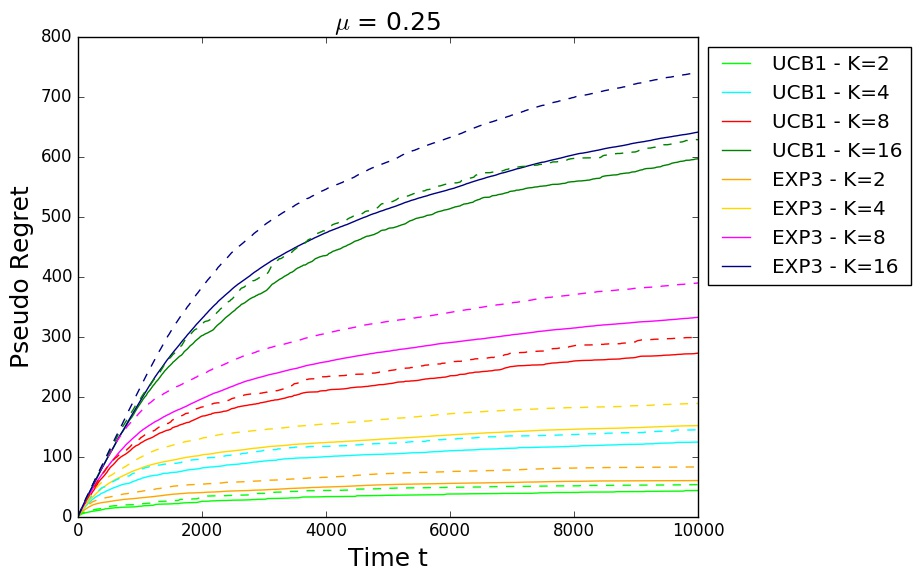
\includegraphics[width=17cm]{fig/000.jpg}
  \caption{\footnotesize Average pseudo regret and average pseudo regret + standard deviation (scribbled line) over 10 runs with $\mu = 0.25$ }
\label{fig:1}
\end{figure}
Figure \ref{fig:1} shows the experiment for $\mu = 0.25$. As evident, the UCB1 and EXP3 algorithm has a very similar performance, however the UCB1 seems to outperform EXP3 slightly on each setting of $K$. It is also clear that the regret increases with the number of arms. The regret increases rapidly for the first few iterations and converges afterwards, as the optimal arm is identified.
\subsection{$\mathbf{\mu^* - \frac{1}{8}}$:}
\begin{figure}[H]
 \centering  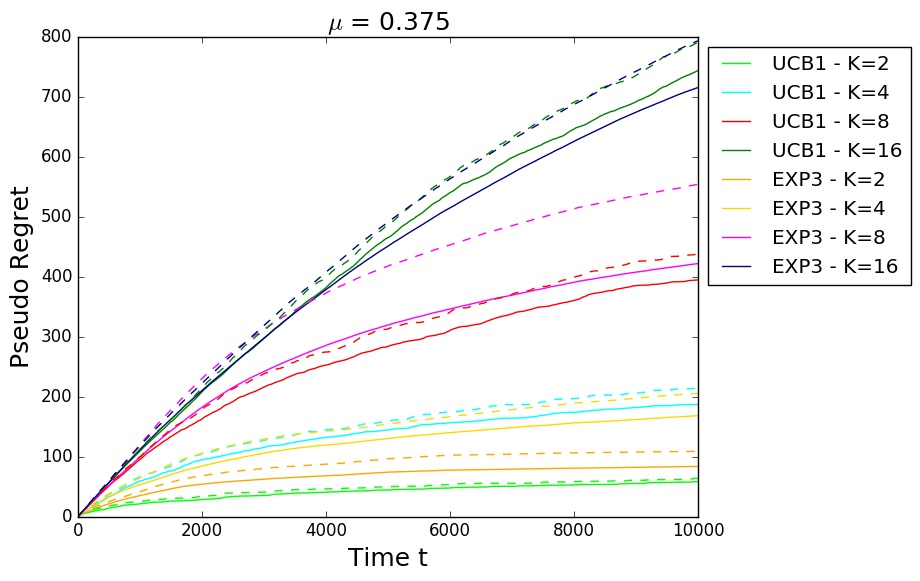
\includegraphics[width=17cm]{fig/222.jpg}
  \caption{\footnotesize Average pseudo regret and average pseudo regret + standard deviation (scribbled line) over 10 runs with $\mu = 0.375$ }
\label{fig:2}
\end{figure}
Figure \ref{fig:2} shows the experiment for $\mu = 0.375$. The pseudo regret is higher than for $\mu = 0.25$, also for larger values of $K$, the regret does not converge as fast. It is also noticeable, that for $K=16$ the pseudo regret is higher for the UCB1 algorithm.
\begin{figure}[H]
 \centering  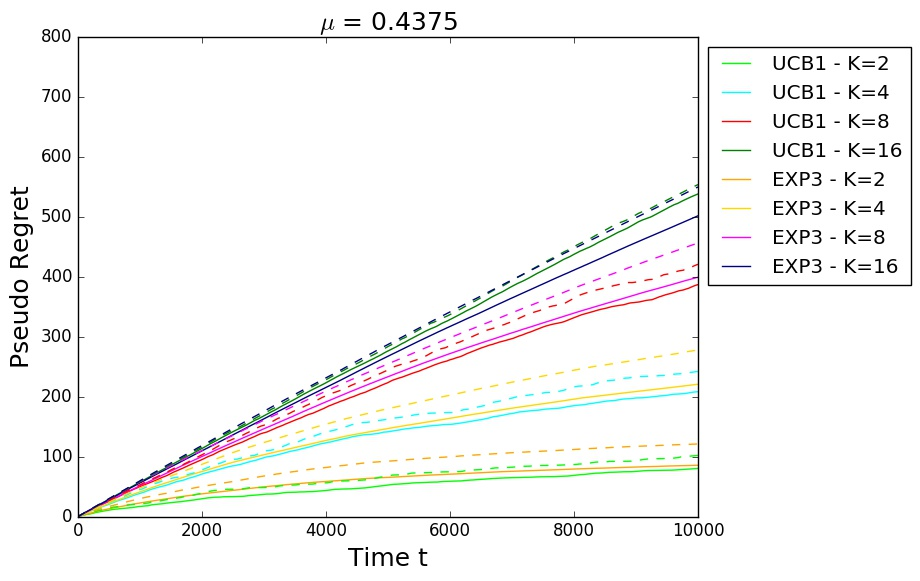
\includegraphics[width=17cm]{fig/333.jpg}
  \caption{\footnotesize Average pseudo regret and average pseudo regret + standard deviation (scribbled line) over 10 runs with $\mu = 0.4375$ }
\subsection{$\mathbf{\mu^* - \frac{1}{16}}$}
\label{fig:3}
\end{figure}
Figure \ref{fig:3} shows the experiment for $\mu = 0.4375$. Interestingly the pseudo regret for $K=16$ is smaller than for the previous settings of $\mu$.
\subsection{Adversarial Sequence}
For this task, we would like to define a sequence of rewards for each arm, such that the performance of the UCB1 algorithm will be bad. The performance of the two algorithms is measure in regret, which is defined as:
\begin{equation}
R_T = \sum\limits_{t=1}^T l_t^{A_t} - \min_{a} \sum\limits_{t=1}^T l_t^{a}
\end{equation}
Below I will describe my idea for the sequence when K=4, however it could be used for any number of K. My initial idea for this task was to define a single arm, say arm $a_0$, which would be optimal, in order to yield the highest regret. The sequence is generated such that after the initialization phase the optimal arm $a_0$ would have the lowest upper confidence bound, and the three other arms would be tied. Such an initialization phase could like like (recall that for the initialization we pick $A_t = t$):
$$
\begin{bmatrix}
a_0 \vline &  0 & 1 & 1 & 1 \\
a_1\vline & 0 & 1 & 0 & 0 \\
a_2\vline & 0 & 0 & 1 & 0 \\
a_3\vline & 0 & 0 & 0 & 1
\end{bmatrix}
$$
For the first iteration after the initialization phase ($t=5$) the prediction will be a random decision between $a_1,a_2,a_3$, therefore we pick the reward sequence of $[1,0,0,0]$, such that we are guaranteed to have a loss i.e pick an arm with zero reward. The upper confidence  bound on the played arm will decrease, and we will now have a tie between the last two arms, if we again pick sequence $[1,0,0,0]$ we are guaranteed to have a loss. For the next iteration there will be a single unplayed arm (any of $a_1,a_2 \text{ or } a_3$) which will have the highest upper confidence bound. Playing this arm will now make the upper confidence bound of the first arm $a_0$ the largest, in which we play the sequence $[0,1,1,1]$ in order to bring back the confidence of the other arms. Initially it appeared that i could play $[1,0,0,0]$ for three iterations (to play the three tied arms) followed by $[0,1,1,1]$ and repeat, but as T increased, the initially proposed pattern did not hold.  \\
Instead i tried a different solution, where we throughout the sequence pick:
$$
\begin{bmatrix}
a_0 \vline &  0 & 1 & 1 & 1 & 0 \dots \\
a_1\vline  &  1 & 0 & 1 & 1 & 1 \dots \\
a_2\vline  &  1 & 1 & 0 & 1 & 1 \dots \\
a_3\vline  &  1 & 1 & 1 & 0 & 1 \dots
\end{bmatrix}
$$
which i somewhat chose because i was not able to get a clear linear regret for the randomized tie breaking and breaking the above sequence using deterministic tie breaking is very straightforward. After initialization, the arms will be tied, if we deterministically pick the first largest arm, then we will pick the arm which has zero reward. When picking the arm, the upper confidence bound of the arm will decrease and we now only consider $a_1,a_2,a_3$, which are tied. Again we pick the first largest, which is $a_2$, which has zero reward and we will continue to do this throughout the whole sequence. The regret of this deterministically tie breaking algorithm is shown in figure \ref{fig:4}
\begin{figure}[H]
 \centering  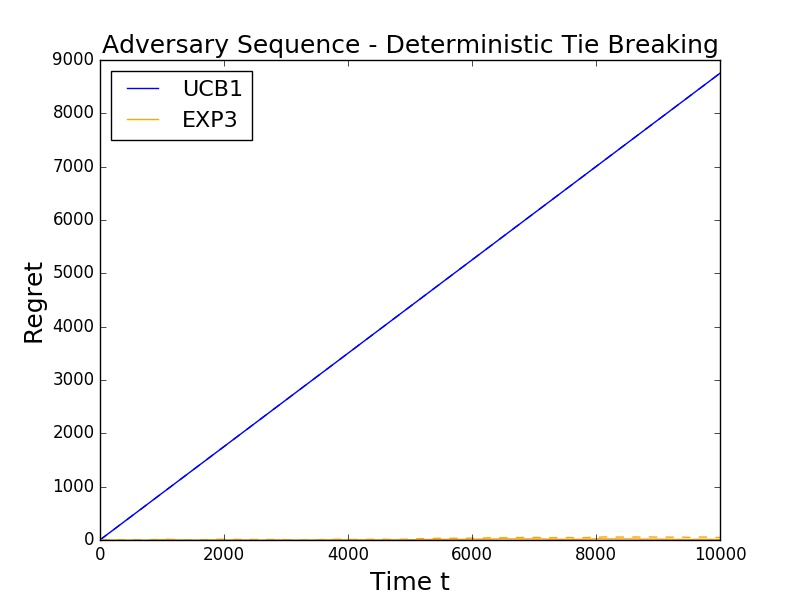
\includegraphics[width=15cm]{fig/newadvseq1.jpg}
  \caption{\footnotesize Average regret and average regret + standard deviation (scribbled line) over 10 runs with $K=7$, using deterministic tie breaking}
\label{fig:4}
\end{figure}
Figure \ref{fig:4} shows the regret of the UCB1 (with deterministic tie breaking) and EXP3 algorithms, plotted as a function of $T$. Thus we were able to break the UCB1 with deterministic tie breaking. It is clear that the EXP3 performed very well on the sequence, which is due to it's probabilistic forecasting, thus not being broken by an adversarial sequence, where UCB1 relies on the sequence to be i.i.d. In figure \ref{fig:5}, the performance of the UCB1 (with random tie breaking) and EXP3 is shown on the same sequence as in figure \ref{fig:4}:
\begin{figure}[H]
 \centering  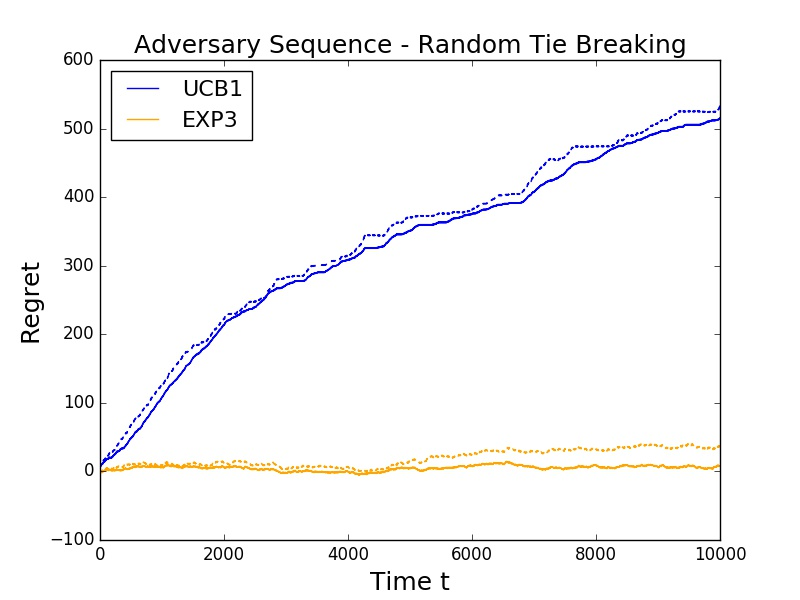
\includegraphics[width=15cm]{fig/newadvseq2.jpg}
  \caption{\footnotesize Average  regret and average pseudo regret + standard deviation (scribbled line) over 10 runs with $K=7$ , using randomized tie breaking}
\label{fig:5}
\end{figure}
Although having a large regret, compared to the EXP3, the UCB1 regret is not linear as we would have wanted.
\end{document}
